%%%% Proceedings format for most of ACM conferences (with the exceptions listed below) and all ICPS volumes.
\documentclass[sigconf]{acmart}
\usepackage{graphicx}
\usepackage{paralist}
\usepackage{booktabs}
\usepackage{tabularx}
\usepackage{url}
\usepackage[hyphenbreaks]{breakurl}

\def\UrlBreaks{\do\/\do-}

%%%% As of March 2017, [siggraph] is no longer used. Please use sigconf (above) for SIGGRAPH conferences.

%%%% Proceedings format for SIGPLAN conferences 
% \documentclass[sigplan, anonymous, review]{acmart}

%%%% Proceedings format for SIGCHI conferences
% \documentclass[sigchi, review]{acmart}

\usepackage{booktabs} % For formal tables


% Copyright
%\setcopyright{none}
%\setcopyright{acmcopyright}
\setcopyright{acmlicensed}
%\setcopyright{rightsretained}
%\setcopyright{usgov}
%\setcopyright{usgovmixed}
%\setcopyright{cagov}
%\setcopyright{cagovmixed}

\copyrightyear{2018} 
\acmYear{2018} 
\setcopyright{iw3c2w3}
\acmConference[WWW'18 Companion]{The 2018 Web Conference Companion}{April 23--27, 2018}{Lyon, France}
%\bookTitle{The 2018 Web Conference Companion, April 23--27, 2018, Lyon, France}
\acmPrice{}
\acmDOI{10.1145/XXXXXX.XXXXXX}
% Do not include "https://doi.org/" thats in the rights form and be sure to update the XXX's with your DOI. 
\acmISBN{978-1-4503-5640-4/18/04.}
% Please include the /18/04. -- its not on the rightsreview forms.

% removes the headers from each page per the preparation instructions, as these are not needed and will be updated with the chairs' actual session names during the pagination/indexing process:
\fancyhead{}

\begin{document}
\title[An Evaluation of Performance and Competition in Customer Services on
  Twitter]{An Evaluation of Performance and Competition in Customer Services on
  Twitter: A UK Telecoms Case Study}
%\titlenote{}
%\subtitle{Extended Abstract}
%\subtitlenote{}

\author{Nabeel Albishry}
\orcid{0000-0002-1231-4491}
\affiliation{%
  \institution{University of Bristol}
  \streetaddress{}
  \city{} 
  \country{United Kingdom}
}
\email{n.albishry@bristol.ac.uk}

\author{Tom Crick}
\orcid{0000-0001-5196-9389}
\affiliation{%
  \institution{Swansea University}
  \streetaddress{}
  \city{} 
  \country{United Kingdom}
}
\email{thomas.crick@swansea.ac.uk}

\author{Theo Tryfonas}
\orcid{0000-0003-4024-8003}
\affiliation{%
  \institution{University of Bristol}
  \streetaddress{}
  \city{} 
  \country{United Kingdom}
}
\email{theo.tryfonas@bristol.ac.uk}

\author{Tesleem Fagade}
%\orcid{}
\affiliation{%
  \institution{University of Bristol}
  \streetaddress{}
  \city{} 
  \country{United Kingdom}
}
\email{tesleem.fagade@bristol.ac.uk}


 
% The default list of authors is too long for headers}
\renewcommand{\shortauthors}{Albishry, Crick, Tryfonas, and Fagade}


\begin{abstract}
With an increasing number of consumers using social media platforms to
share both their satisfaction and displeasure about the products and
services they use every day, organisations with a customer service
focus are recognising the importance of rapid -- and genuine -- online
engagement with their customers. In turn, consumers increasingly judge
organisations on the quality of customer service and degree of
responsiveness to online queries. This paper presents an extensible
framework for evaluating direct engagements of customer service teams
with customers on Twitter. Furthermore, this framework provides the
capability to measure and analyse indirect engagement with industry
sector rivals, especially their patterns, frequency and intensity. By
applying graph analysis to these Twitter interactions, our framework
generates various analytical measures and visual representations,
exemplified through a case study based on seven major UK telecoms
companies. With a dataset consisting of 15,000 tweets and 3,500 user
profiles, the results provide sustained evidence for indirect
engagements between business rivals, with customer queries acting as a
trigger for intense competition between companies based in the same
industry sub-domain.
\end{abstract}

\begin{CCSXML}
<ccs2012>
<concept>
<concept_id>10003120.10003130.10003131.10003292</concept_id>
<concept_desc>Human-centered computing~Social networks</concept_desc>
<concept_significance>500</concept_significance>
</concept>
% <concept>
% <concept_id>10003120.10003130.10003131.10011761</concept_id>
% <concept_desc>Human-centered computing~Social media</concept_desc>
% <concept_significance>500</concept_significance>
% </concept>
<concept>
<concept_id>10003120.10003130.10003134.10003293</concept_id>
<concept_desc>Human-centered computing~Social network analysis</concept_desc>
<concept_significance>500</concept_significance>
</concept>
<concept>
<concept_id>10003120.10003130.10003233.10010519</concept_id>
<concept_desc>Human-centered computing~Social networking sites</concept_desc>
<concept_significance>500</concept_significance>
</concept>
<concept>
<concept_id>10003120.10003145.10003147.10010923</concept_id>
<concept_desc>Human-centered computing~Information visualization</concept_desc>
<concept_significance>100</concept_significance>
</concept>
<concept>
<concept_id>10010405.10010406.10010412.10011712</concept_id>
<concept_desc>Applied computing~Business intelligence</concept_desc>
<concept_significance>500</concept_significance>
</concept>
<concept>
<concept_id>10010147.10010178.10010179.10003352</concept_id>
<concept_desc>Computing methodologies~Information extraction</concept_desc>
<concept_significance>300</concept_significance>
</concept>
</ccs2012>
\end{CCSXML}

\ccsdesc[500]{Human-centered computing~Social networks}
%\ccsdesc[500]{Human-centered computing~Social media}
\ccsdesc[500]{Human-centered computing~Social network analysis}
\ccsdesc[500]{Human-centered computing~Social networking sites}
\ccsdesc[100]{Human-centered computing~Information visualization}
\ccsdesc[500]{Applied computing~Business intelligence}
\ccsdesc[300]{Computing methodologies~Information extraction}

\keywords{Customer services; reply chains; graph
  construction; social network analysis; Twitter; social media}

\maketitle

\section{Introduction}\label{intro}

The online news and social networking service Twitter has become one
of the most popular social platforms for a variety of demographics
across the world. It provides a rich, constantly updating, corpus of
big social data to study a range of complex socio-cultural issues,
from life event detection~\cite{blamey-et-al-2013} and identifying
multilingual communities~\cite{albishry-et-al:iccci2017}, through to
sentiment classification~\cite{blamey-et-al-2012} and providing deeper
insight into personality and
behaviour~\cite{mostafa-et-al-ai2016}. Unsurprisingly, Twitter is
increasingly being used by organisations to communicate with their
customers, due to the fast and convenient medium of
engagement~\cite{ma-et-al:2015}, using a variety of sophisticated
human and automated
approaches~\cite{verhagen-et-al:2014,xu-et-al:2017}. In 2016, a survey
was carried out on 5,450 people who follow small or medium-sized
enterprises (SME) on Twitter~\cite{Twitter2016}; the key results show
that 83\% of people that received a reply felt better about the SME,
and 68.7\% have made at least one purchase from an SME because of
Twitter.

The medium can thus serve as an indicator to underlying issues of
performance, management and even strategic
matters~\cite{gregoire-et-al:2015}; in many instances, the majority of
complaints deal with product and service-related
issues~\cite{einwiller+steilen:2015}. Many studies have been conducted
to explore aspects of customer services experiences in various
business domains, such as travel and
telecoms~\cite{Shakeel2017,Zhang2016,Wattimena2017,misopoulos-et-al:2014,Khatoon2017}.
News agencies are not far from social media analysis, using it to
uncover users' interests so they can provide more focused
contents~\cite{Nigam2016}. While various domains have long applied
network analysis techniques -- such as for crime detection and
prevention~\cite{oatley+crick:2015,oatley-et-al:dasc2015} -- only
recently has work has been conducted to see how users relate to brands
via network structures~\cite{Cutler2017}, how information shared by
companies disseminate and their types~\cite{Piccialli2017}, and what
type of engagements from companies was found to be of effect on
customers perception of the brand~\cite{Ibrahim2017}. A common
approach in conducting such studies has been to use sentiment
analysis, mainly to measure consumer's perception and
satisfaction~\cite{Zhang2016,Al-Hussaini2017}.

However, the novel framework presented here aims to provide
quantitative insights that can produce a more holistic view of
customer service Twitter accounts and their interactions. Rather than
focusing on individual posts and their sentiment, the framework helps
in identifying complaint conversations that can be exploited by other
business rivals, to be interrogated further by analysts or decision
makers. With the high volume of activity on Twitter, the framework
focuses on detecting possible key issues by using the connected
component feature of graph to identify problematic conversations for
further analysis. Furthermore, by using streaming and RESTful data,
this approach can be applied to live data to catch problematic
conversations before they reach certain thresholds.

The remainder of this paper is organised as follows: in
Sections~\ref{casestudy} we introduce the case study of the UK
telecoms sector; in Section~\ref{method} our methodology for this
project; Section~\ref{results} presents the results and key visual
representations; Section~\ref{discussion} provides the main
discussion; Section~\ref{conclusions} concludes the paper with a
discussion of potential extensions and wider application of this work.

\section{Case Study: UK Telecoms Sector}\label{casestudy}

Most UK households have access to both fixed broadband and a
smartphone, with consumers moving seamlessly between fixed and mobile
connections. This has been driven by the growing take-up of superfast
broadband services, with the proportion of UK households with fixed
broadband increasing to 82\% in 2017, with telecoms services rising to
3.8\% of total household spend. With the increasing convergence of
mobile and Wi-Fi connectivity, many customers in the UK have switched
from pay-as-you-go tariffs to pay-monthly tariffs in 2016, and nearly
two-thirds of mobile connections were 4G-enabled at the end of
2016. Consumers are also using these networks more -- average data use
per fixed line residential broadband connection increased by 36\% year
on year to 132GB in June 2016, and average data use per mobile
connection increased by 44\% to 1.3GB~\cite{ofcom:2017}. The UK
telecoms sector has continued to grow rapidly over the past five
years, with total sector revenues in 2016 of \pounds35.6bn, including
mobile retail revenues of \pounds15.3bn~\cite{ofcom:2017}.

There are four main fixed broadband network operators in the UK: BT,
Sky, TalkTalk and Virgin Media; alongside the incumbent BT,
alternative providers compete in the retail provision of fixed
services (including telephony and broadband), as well as other
operators using a variety of wholesale inputs purchased from BT and
resellers. There are currently four main mobile network operators
(MNOs) in the UK (with 2017 subscriber numbers): BT/EE (29.8m),
O2/Telef\`{o}nica (25m), Vodafone (17.6m), and Three/H3G (12.01m);
there are also several mobile virtual network operators (MVNOs),
including Virgin Mobile (via EE, 3m), giffgaff (via O2, 420,000) and
Sky Mobile (via O2, 335,000)~\cite{ecdpr:2017}.


\section{Methodology}\label{method}

The dataset contains tweets and related replies for seven well-known
UK telecoms companies: BT, EE\footnote{BT's acquisition of EE was
completed in 2016; the merger did not materially increase EE's market
share, but as a result of the merger EE's useable spectrum share
increased. There have been no other significant new entrants or
changes in market share since.}, giffgaff, O2, Sky, Virgin Media and
Vodafone. The choices were intended to represent companies of various
sizes, history and range of services provided. While a few companies
only had one account on Twitter, some of them have multiple
accounts alongside the primary Twitter account; in those instances,
the dedicated customer services accounts were indicated in the
biography of the company's other accounts. Therefore, as the focus of
the study is on customer services on Twitter, data were collected from
either the company's primary account or its dedicated customer services
one (N.B. names throughout the paper will refer to Twitter account handles
rather than official company trading names).

Inspired by the approach taken by Cogan et al.~\cite{Cogan2012}, this
study consists of two main steps: the data collection phases and the
graph construction. The data collection phase runs iteratively to obtain
reply chains, process them and store them in a database. Once the data
collection phase is completed, a large graph that includes all reply
nodes and edges is constructed to conduct the initial analysis. The
NetworkX Python package~\cite{Hagberg2008} was used for the graph
construction, while Gephi~\cite{Bastian2009} provided a range of tools
for visualisation.

% \begin{figure}[htb]
% \centering
% 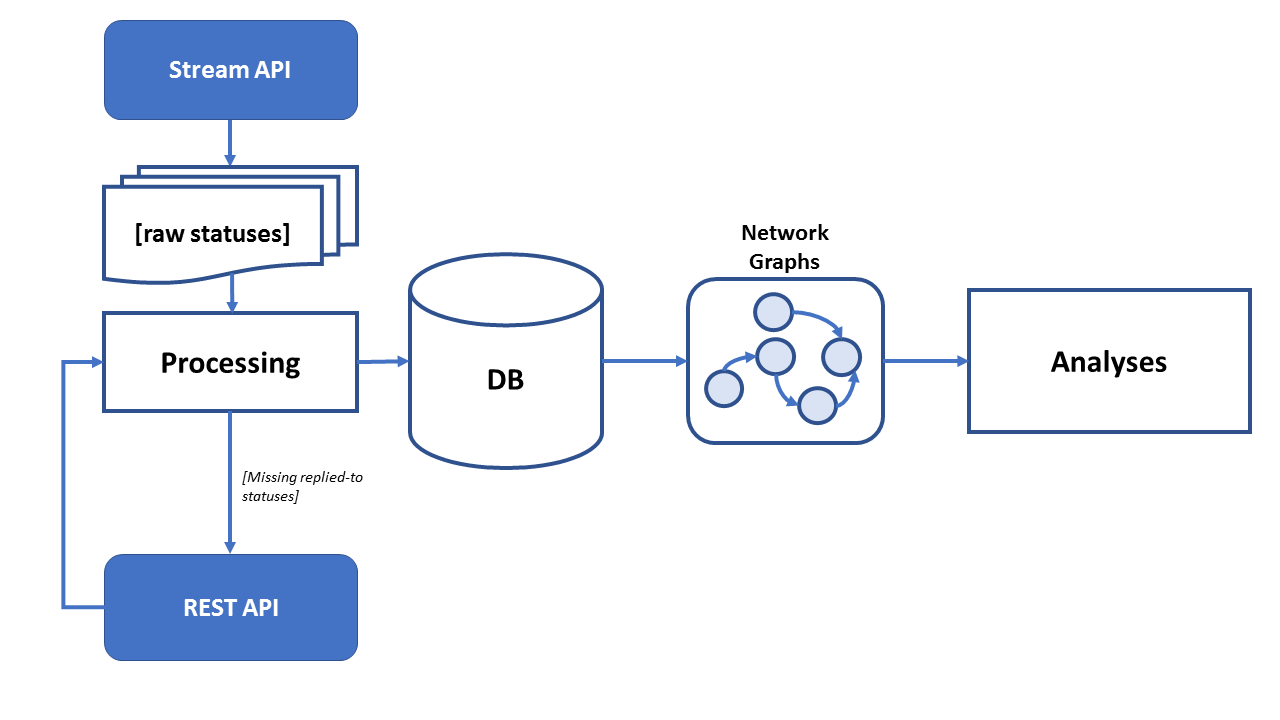
\includegraphics[width=\columnwidth]{images/frameworkstructure.png}
% \caption{Overall framework structure}
% \label{fig:frameworkstructure}
% \end{figure}

\subsection{Streaming}

To ensure we were able to collect as much data as possible, the data
collection comprised of three steps. First, a stream endpoint is
opened to catch activities of accounts under investigation, those
accounts will be referred to as `CS' (customer service)
accounts. The Twitter Streaming
API\footnote{\url{https://developer.twitter.com/en/docs}} is designed
to return tweets created by the user, their retweets, replies directed
to their tweets, and retweets of their tweets. However, the stream
does not include tweets mentioning the user, and replies/retweets by
protected users.

\subsection{Reply Chains}

Returned statuses from the Streaming API may represent reply-to
statuses that have not been collected previously. It was found that
most missing statuses were either posted before the data collection
started, were mentions, or that the user account is protected. This
issue could have a significant impact on the quality of the analysis;
therefore, once statuses are returned from the stream endpoint, their
type is checked first (tweet, retweet, etc). If status is a reply, the
ID of the status to which it was replying is extracted from
{\emph{in\_reply\_to\_status\_id}}. Then, using the extracted ID, we
check if the replied-to status has already been collected and present
in the dataset or not. If not, the REST API is then used to collect
them. This process runs recursively for newly-collected replies until
no further replies are available. Unavailable statuses are often
results from either deletion or protected accounts.

An analysis of changes on the graph after the second phase of data
collection shows that there were increases in the number of nodes and
edges by 43\% and 62\%, respectively. This increase in connections has
resulted in merging 176 conversations into others, which improved
connectivity of the graph and, thus, the accuracy of the dependent
analyses.

% \begin{figure}[htb]
% \centering
% 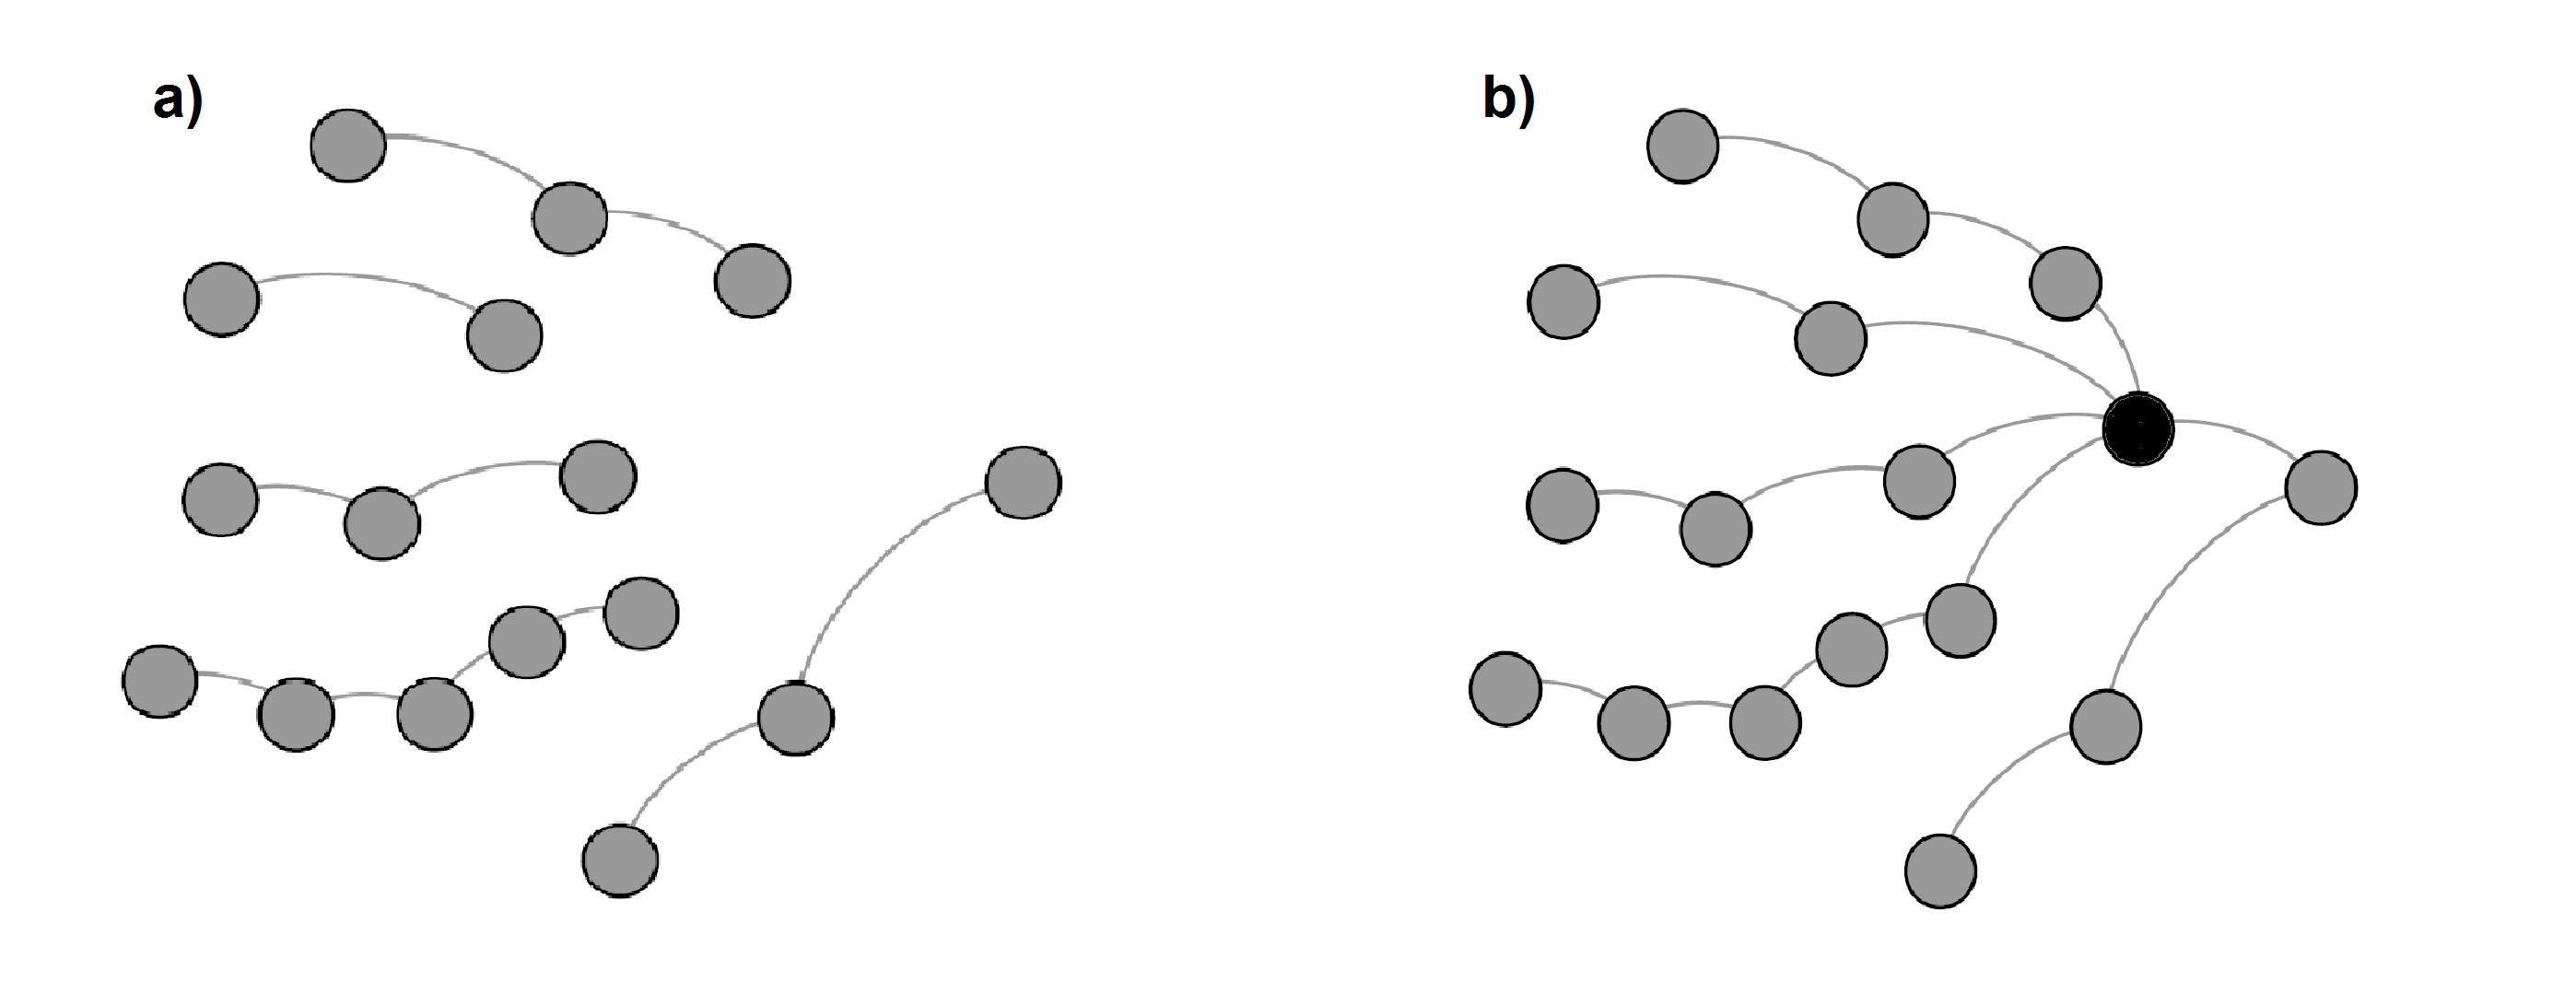
\includegraphics[width=\columnwidth]{images/datacollectionphases.png}
% \caption{(a) First phase of data collection and (b) second phase of data
% collection}
% \label{fig:datacollectionphases}
% \end{figure}


\subsection{Graph Construction}

The main data structure of conversations on Twitter suggests
status-to-status {\footnote{We use `status' to refer to any type of post, tweet,
retweet, reply, or quote.}} relationship. In graph concept, statuses
represent nodes that are linked by directed edges. Therefore, the
study follows a graph construction approach in conducting analysis and
produces three graphs. First, {\emph{base}} graph is constructed to
capture structure of the dataset, i.e. status-to-status.  Then, from
the base graph, it generates two graphs: the {\emph{Users} graph to
examine the user-to-user direct engagements, and the {\emph{Coexistence}}
graph to uncover and examine indirect engagements amongst rivals.

\subsubsection{Base Graph}

Once the data are collected, a base graph is generated containing all
replies and all related information. Nodes represent status IDs, while
edges indicate replying direction; other information is added as
attributes to nodes. The information used in this study are
{\emph{screen\_name}} of the user, {\emph{timestamp}} of the reply,
{\emph{text}}, and {\emph{CS}}. The additional {\emph{CS}} value is a
binary digit set to distinguish accounts -- it is set to 1 if the status
belongs to one of the CS accounts, otherwise it is 0. This value is
required to eliminate the need for user checks in forthcoming
analyses. Figure~\ref{fig:replychaingraph} illustrates the conceptual base
graph. As a reply can be directed to only one other status, no edge is
expected to have weight value other than 1, and no reply status can
have outdegree greater than 1. Nodes with 0 outdegree can be either a
root node, or it is directed to unavailable statuses. On the other
hand, indegree in this graph indicates the number of replies directed to
the status node; hence, 0 indegree distinguishes leaf nodes. Special case
nodes are those with indegree and outdegree equal to 0; these are
isolated/floating nodes and must be removed before we perform the
analysis -- these nodes do not benefit the analysis as they are not
part of a conversation. Furthermore, they will be seen as connected
component by themselves, which impacts upon the accuracy of results.

\begin{figure}[htb]
\centering
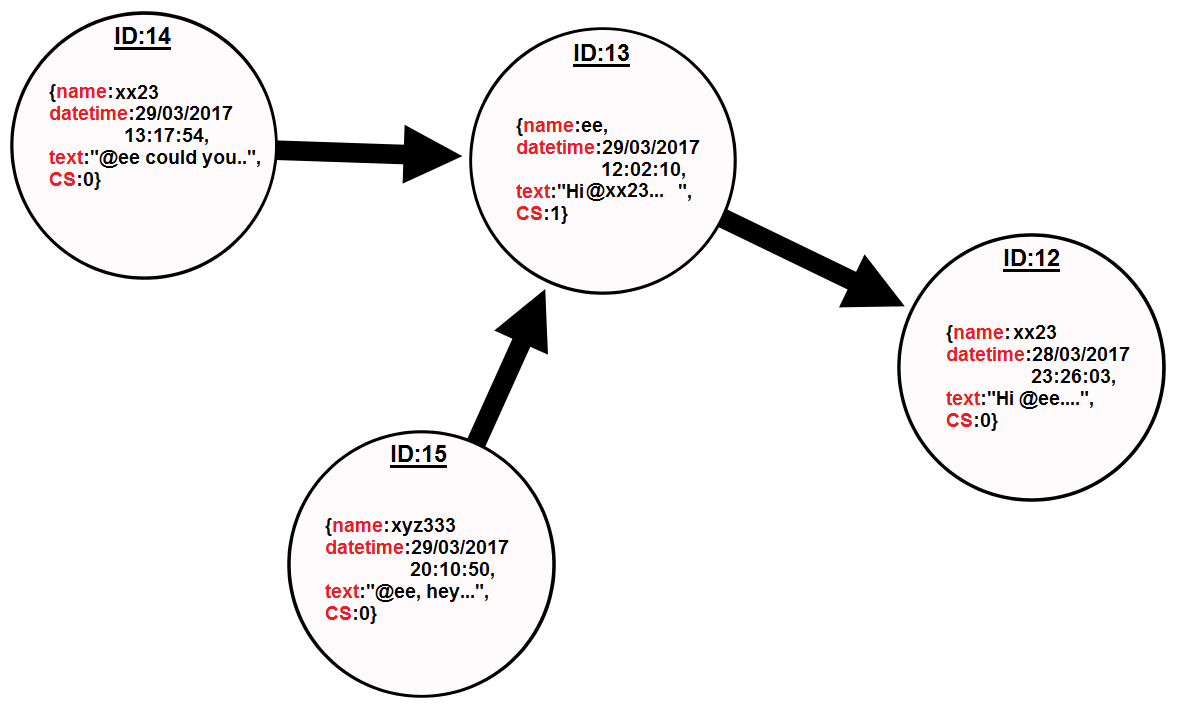
\includegraphics[width=\columnwidth]{images/replychaingraph.png}
\caption{Example of a reply chain graph}
\label{fig:replychaingraph}
\end{figure}

\subsubsection{Users' Graph}

Because most of the analysis focus on relationships between reply
posts, they were applied on the base graph. Nevertheless, to allow
examination of the relationships between users, another graph is
generated from the base graph. This process is carried out by
iterating through edges linking reply posts, extracting users'
information, and constructing users graph accordingly. In the context
of this study, only two attributes are used: screen names and
`CS' values. While nodes represent screen names, `CS' values
are attached to nodes as attribute. For edges, their weights indicate
number of replies sent from origin node (sender) to target node
(receiver); therefore, the user graph is directed. Applying this
process on the example in Figure~\ref{fig:replychaingraph} results in
the users graph in Figure~\ref{fig:usersgraph}.

\begin{figure}[htb]
\centering
\includegraphics[width=\columnwidth]{images/usersgraph.png}
\caption{Example of users' graph extracted from base graph}
\label{fig:usersgraph}
\end{figure}

To examine relationships between users, five network graph properties
are measured. There were no special case nodes or edges in this graph,
as observed in the base graph. For edges, their orientation indicate
direction of replies, while weight reflects number of replies on the
edge.  Node indegree reflect number of users that have sent reply to
the node, and outdegree indicates the number of users that have
received reply from the node. Also, weighted measure of indegree and
outdegree indicate total received and sent replies, respectively.

%Graph properties that are used in
%analysing this graph and their contextual interpretations are shown in
%Table~\ref{tbl:uucentralitymeasuresinter}.

%\begin{table}[!h]
%\centering
%\begin{tabularx}{\columnwidth}{lX}
%\toprule
%\textbf{Measure} & \textbf{Interpretation} \\ 
%\midrule
%{\emph{Indegree}} & Number of users that sent reply to the node \\
%{\emph{Weighted Indegree}} & Total number of received replies \\
%{\emph{Outdegree}} & Number of users that have received a reply from
 %                    the node \\ 
%{\emph{Weighted Outdegree}} & Total number of sent replies \\
%{\emph{Edge Weight}}& Number of replies between the connecting nodes\\
%\bottomrule
%\end{tabularx}
%\caption{User-user centrality measures interpretation}
%\label{tbl:uucentralitymeasuresinter}
%\end{table}

\subsubsection{Connected Components}

Reply conversations in the base graph are not interconnected, which
implies that the graph actually consists of many subgraphs, or
`connected components'. Since nodes include screen names, those
components can be linked to CS accounts. Then, they are used to
measure the size of conversation, their depths, and to identify shared
conversations between the CS accounts. In the base graph, the number
of connected components reflect the number of conversations. Therefore, in
the base graph many components should be expected, depending on
activity of the CS accounts and their audience.

To find conversations for a specific CS account, the search run
through all components; in each component, the process iterates
through nodes and examine the {\emph{name}} attribute. Once a match is
found, the search process stops and the identified component is either
analysed on the fly, or returned for further analysis. Additionally,
some of those components will be used to construct the coexistence
graph, as covered next.

\subsubsection{Coexistence Graph}

As mentioned previously, this graph aims to measure the indirect
engagements amongst the CS accounts. Therefore, all components in the
base graph are processed in turn to find which CS accounts
appeared. For each component, name attributes for nodes with CS value
equal to 1 are extracted.  If more than one CS account was found,
those accounts are used to created nodes and edges for the coexistence
graph. Thus, nodes are generated from CS names, and edges indicate
common conversation between linked nodes. Subsequently, if the edge
already exists, its weight is increased.  For an illustration of this
process, see Figure~\ref{fig:ccmethod} and
Figure~\ref{fig:coexistencegraph2} to exemplify three common
components and the resultant coexistence graph.

\begin{figure}[htb]
\centering
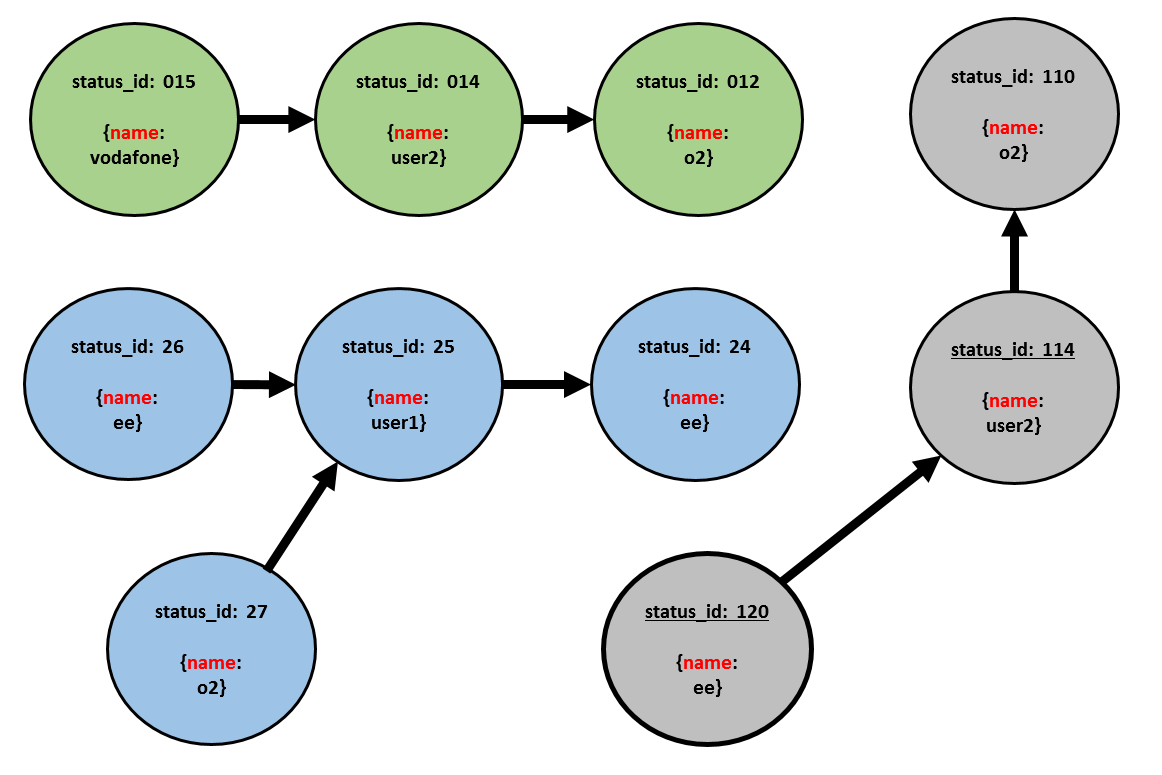
\includegraphics[width=\columnwidth]{images/ccmethod.png}
\caption{Example of common components (only names included for clarity)}
\label{fig:ccmethod}
\end{figure}

\begin{figure}[htb]
\centering
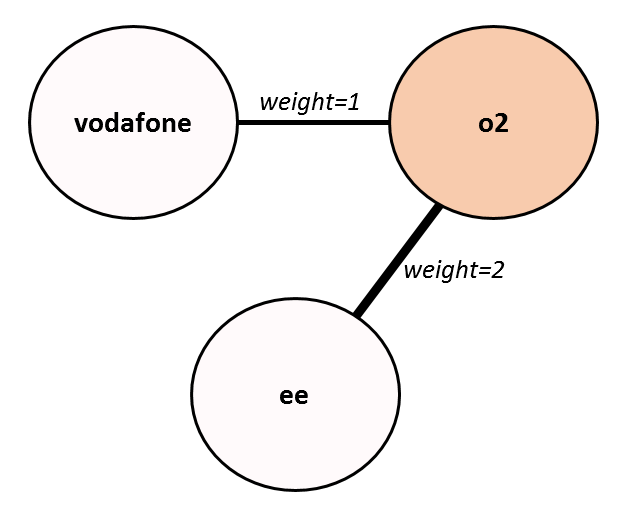
\includegraphics[width=0.8\columnwidth]{images/coexistencegraph2.png}
\caption{An example coexistence graph}
\label{fig:coexistencegraph2}
\end{figure}

\section{Results}\label{results}

%\subsection{Accounts Activity}

%The initial step was to measure accounts activity in terms of
%posting, such as tweeting and replying. Total activity reflects 
%accumulated statuses throughout the data collection phases, from 
%the Streaming and REST APIs. As shown in Figure~\ref{fig:totalactivity}, 
%{\emph{@virginmedia}} was found the most active CS account by 
%farm. 

%As the focus of this section is on customer service, it is 
%necessary to investigate post types to examine the purposes of 
%these accounts. The result shows that replies were at least 83.5\% 
%of accounts activity. This confirms that all chosen accounts are 
%primarily used to interact with customers, handling requests and 
%queries. Therefore, the resulting analyses will be based on replies only.

%\begin{figure}[htb]
%\centering
%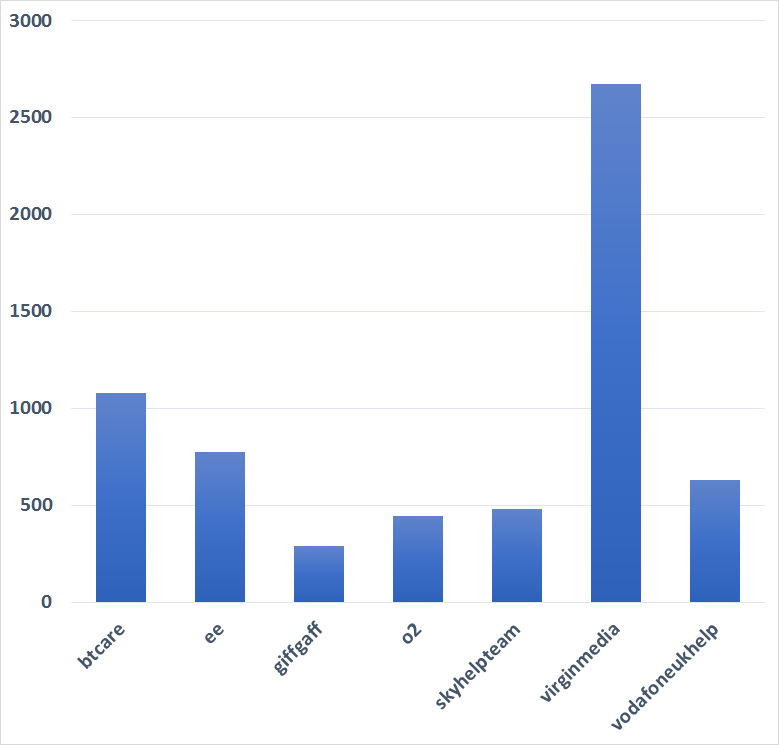
\includegraphics[width=\columnwidth]{images/totalactivity.png}
%\caption{Total activity}
%\label{fig:totalactivity}
%\end{figure}

% \begin{figure}[htb]
% \centering
% 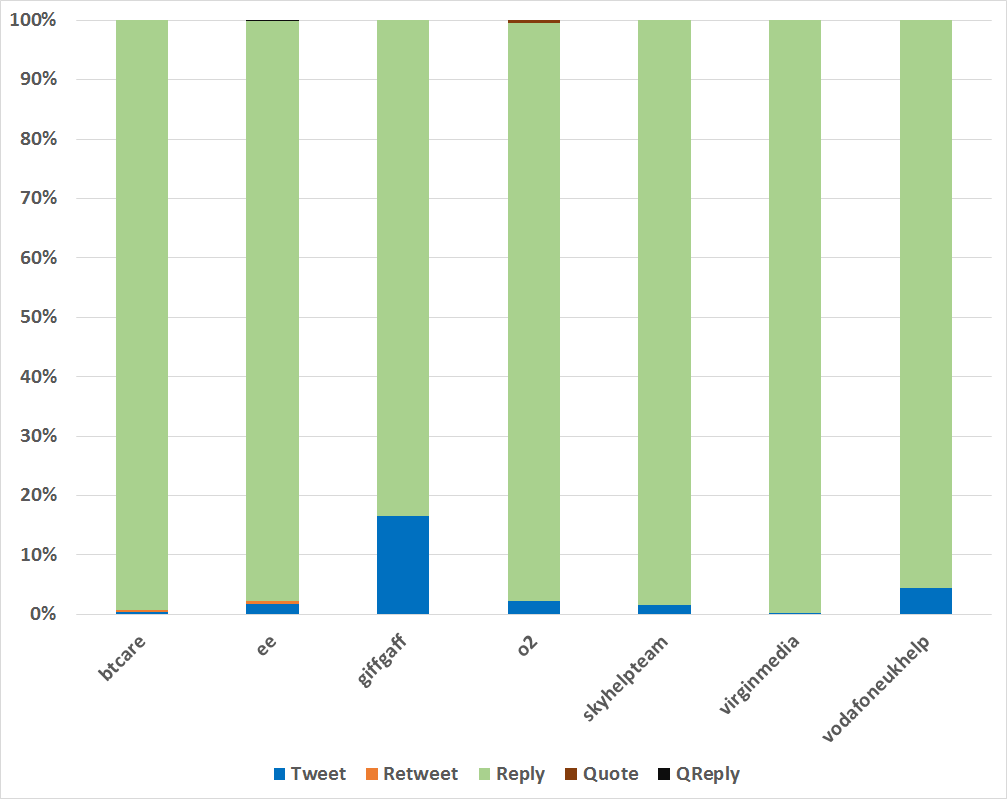
\includegraphics[width=\columnwidth]{images/accountsactivity.png}
% \caption{Accounts activity}
% \label{fig:accountsactivity}
% \end{figure}

\subsection{Delay}\label{results_delay}

Calculating delays is important to provide insight on the performance
of the various CS teams. As reply nodes in the base graph include
timestamp attribute, measuring delay is achieved by calculating time
differences between end nodes on each edge. Table~\ref{tbl:delaystats}
shows key statistics for CS account delays; interestingly,
{\emph{@skyhelpteam}} was found to have an average delay of 45.04
hours, although the rest of the CS accounts' delay ranged between 1.14
and 3.34 hours.

% \begin{figure}[htb]
% \centering
% 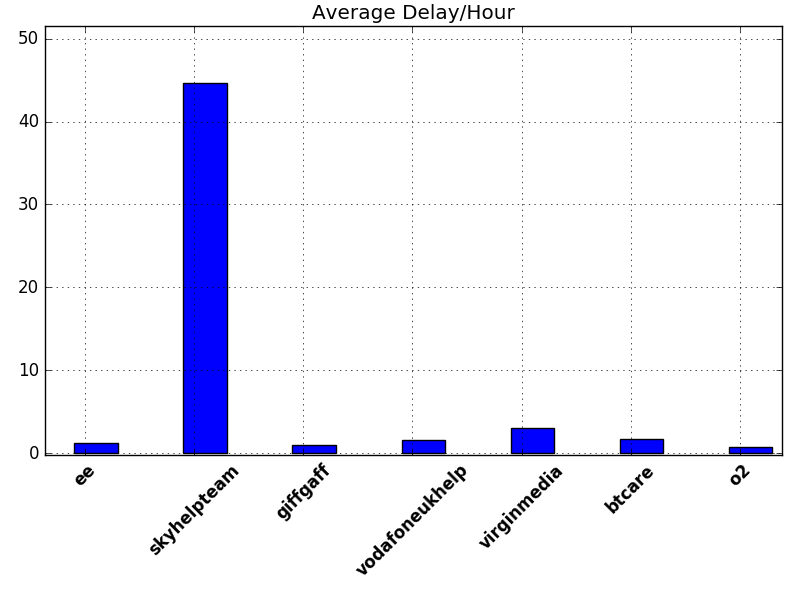
\includegraphics[width=\columnwidth]{images/delaymeans.png}
% \caption{Delay means for CS accounts}
% \label{fig:delaymeans}
% \end{figure}

\begin{table}[!h]
\centering
\begin{tabularx}{\columnwidth}{lrrrr}
\toprule
\textbf{Account} & \textbf{mean} & \textbf{stdev} & \textbf{max} & \textbf{min(sec)} \\ 
\midrule
{\emph{btcare}} & 2.04 & 16.11 & 572.46 & 38\\
{\emph{ee}} & 1.46 & 3.39 & 19.28 & 27\\
{\emph{giffgagg}} & 1.22 & 10.25 & 159.97 & 73\\ 
{\emph{o2}} & 1.14 & 2.66 & 22.48 & 58\\
{\emph{skyhelpteam}} & 45.04 & 49.16 & 117.21 & 44\\
{\emph{virginmedia}} & 3.34 & 9.25 & 263.98 & 22\\
{\emph{vodaphoneukhelp}} & 1.92 & 5.01 & 76.51 & 50\\
\bottomrule
\end{tabularx}
\caption{Summary delays statistics}
\label{tbl:delaystats}
\end{table}

\subsection{Interaction and Users}

%Although the indicated ``working hours'' of CS accounts is important
%to evaluate activity, it is valuable to measure posts that are
%directed to those accounts from other users and examine them in line
%with CS accounts. Audience and their relations with the accounts can
%be analysed directly from the base graph (i.e. post-post). However, as
%user details are embedded inside post nodes, observing such
%relationships will not simple task to accomplish. Therefore, a

To measure interaction amongst users, user-user graphs were built 
from the base graph.; the resultant graph contains 3,521 user nodes 
and 5,938 edges. %as shown in Figure~\ref{fig:userusergraph}. 
Although edges in the base graph cannot
have a weight greater than one, edge weight in the users graph includes all 
replies from one user to another. Therefore, the number of nodes and edges
in the users graph is lower that those in the base graph.

%\begin{figure}[htb]
%\centering
%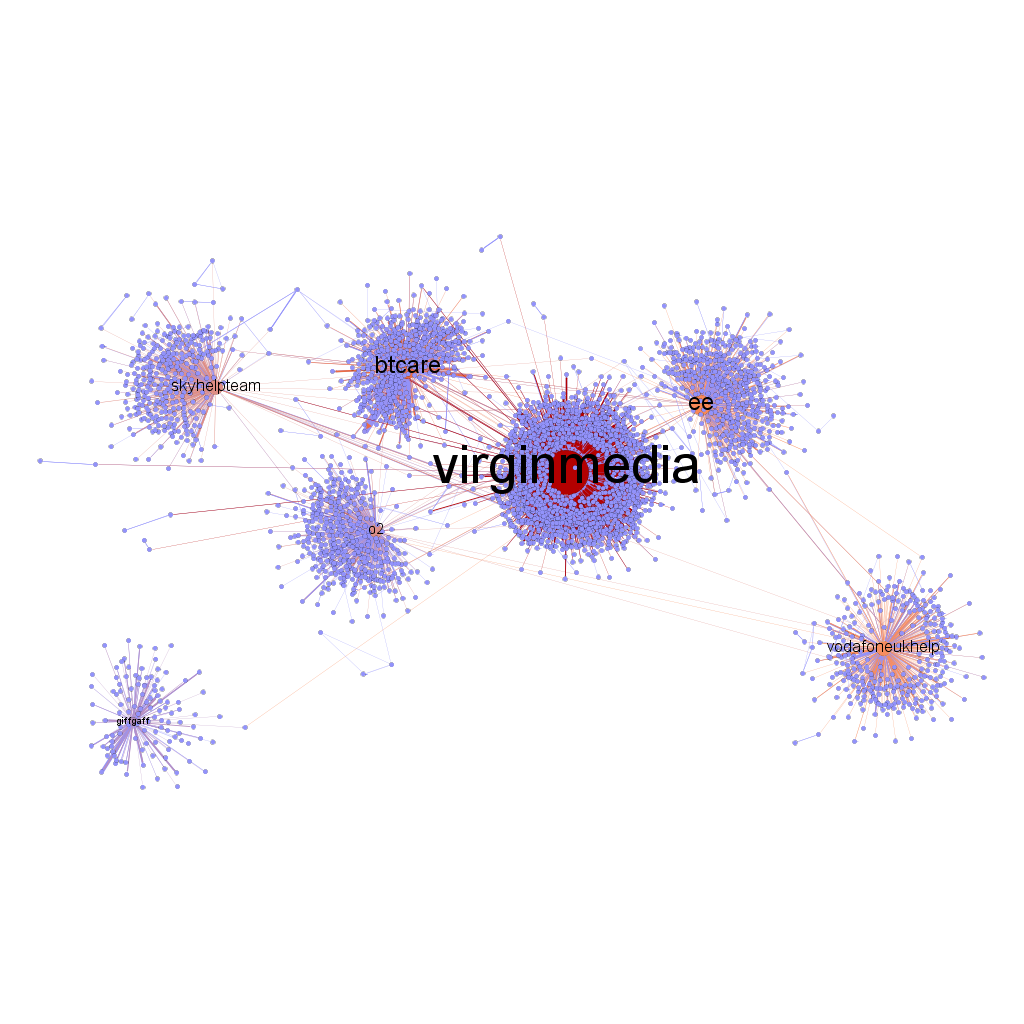
\includegraphics[width=\columnwidth]{images/userusergraph.png}
%\caption{User-user graph}
%\label{fig:userusergraph}
%\end{figure}

Properties of the users graph are presented below in
Table~\ref{tbl:uucentralitymeasures}; the table show that
{\emph{@virginmedia}} received that highest number of replies from 866
users with an average of 3.05 per user. Also, the same account scored
highest in the number of recipients. The difference between indegrees
and outdegrees shows that apart from {\emph{@o2}}, all accounts have
outdegrees bigger that their indegrees. Additionally, the total number
of sent replies is found to be more than the number of received
replies; this may reflect that those replies were directed to
non-reply posts.

\begin{table}[!h]
\centering
\begin{tabularx}{\columnwidth}{l|rrc|rrc}
\toprule
\textbf{Measure} & \textbf{ind} & \textbf{w.ind} & \textbf{\%} & \textbf{out} & \textbf{w.oud} & \textbf{\%}\\ 
\midrule
{\emph{btcare}} & 330 & 995 & 3.02 & 485 & 1317 & 2.72\\
{\emph{ee}} & 247 & 432 & 1.75 & 470 & 778 & 1.66 \\
{\emph{giffgagg}} & 77 & 209 & 2.71 & 102 & 247 & 2.42 \\ 
{\emph{o2}} & 293 & 463 & 1.58 & 260 & 479 & 1.84 \\
{\emph{skyhelpteam}} & 147 & 254 & 1.73 & 305 & 504 & 1.65\\
{\emph{virginmedia}} & 866 & 2645 & 3.05 & 1215 & 3421 & 2.82\\
{\emph{vodaphoneukhelp}} & 166 & 403 & 2.43 & 302 & 660 & 2.19\\
\bottomrule
\end{tabularx}
\caption{Centrality measures of user-user graph}
\label{tbl:uucentralitymeasures}
\end{table}


\subsection{Conversation Components}

As discussed in the methodology, each connected component in the base
graph represent a conversation component that includes related
replies. In this dataset, there were 3,289 conversation components
with various number of replies. Observations of their sizes shows that
the smallest component consists of one post, while the largest
component contains 81 posts. The number of one-post components was
102, and they were all found to belong to CS accounts. Examining those
singular components revealed that they were either original tweets
that have not received replies, or replies to unavailable statuses. As
covered earlier, unavailable replies are those that could not be
captured due to a deletion or the posting account being
protected. Because they do not have any length, and hence do not
represent conversation, single-node components have been excluded from
forthcoming analyses.

Additionally, the majority components were found to have two
nodes. Those components were 1,188 and the orientation of their edge's
direction suggest that most of these communications were from CS
accounts and directed to customer's post. However, 25 of those
conversations were initiated by customers.  As they are two-node
components, it seems that those posts have not been answered by the
relevant CS account. Although other means of communications could have
been used, such as direct messages, there were no visible sign of
further interaction.

% \begin{figure}[htb]
% \centering
% 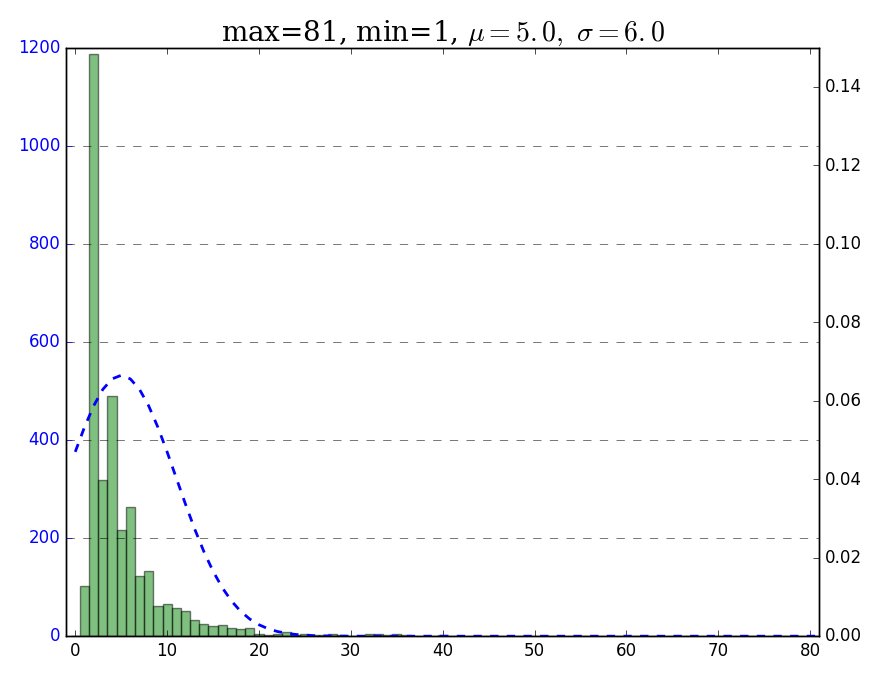
\includegraphics[width=\columnwidth]{images/ccsizes.png}
% \caption{Connected component sizes}
% \label{fig:ccsizes}
% \end{figure}

\subsection{Component Size and Longest Path}

It is important to note that the size of connected components does not
necessarily reflect length of conversations, although there is a
strong correlation between size of component and length of its longest
path (0.88). As can be seen in Figure~\ref{fig:ccsizepaths}, many
components measures are positioned in a near-perfect diagonal line;
interestingly, the longest path in the biggest component (81
nodes/posts) was only 1.

\begin{figure}[htb]
\centering
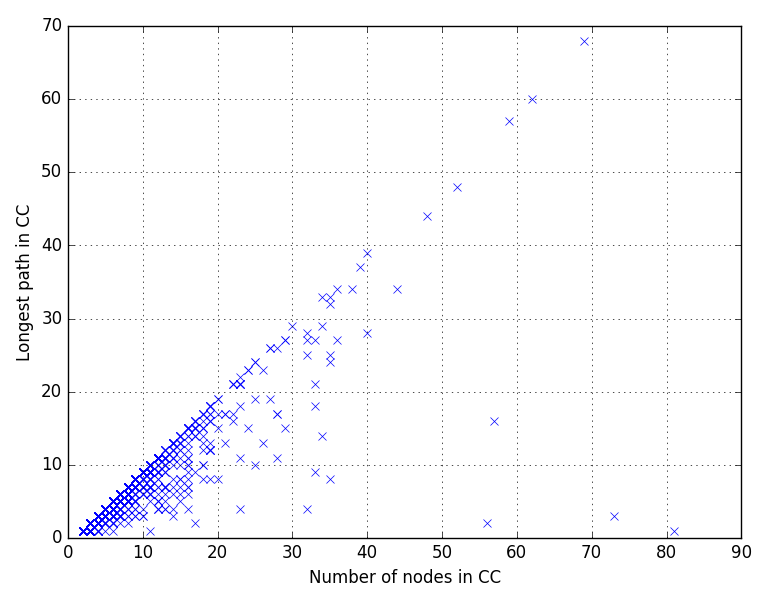
\includegraphics[width=\columnwidth]{images/ccsizepaths.png}
\caption{Size of components and their longest paths}
\label{fig:ccsizepaths}
\end{figure}

To illustrate properties of connected components, the largest 20
components were chosen for visualisation, as shown in
Figure~\ref{fig:20ccpostpostgraph}. The findings show that components
with very high variations in indegree amongst their nodes mostly
originate from CS accounts. An example of this claim is illustrated by
the three big components in the figure; when observed, they were found
to featuring advertising tweets that had received too many replies
from Twitter users.  For example, the root node in the biggest
component was a post by {\emph{@o2}} that has indegree of 80, and all
connected nodes have indegree of zero, i.e. they were not answered. On
the other hand, the longest path component was ranked the third
biggest component. It was found with a single leaf, and all other
nodes along the path were found with indegree=1 and outdegree=1,
forming what we call a {\emph{simple chain}}, uniquely coloured in
Figure~\ref{fig:20ccpostpostgraph}. Additionally, 15 of those
components were found to have originated from customer accounts, and
they all take a semi-simple chain as they feature some branches.

\begin{figure*}[htb]
\centering
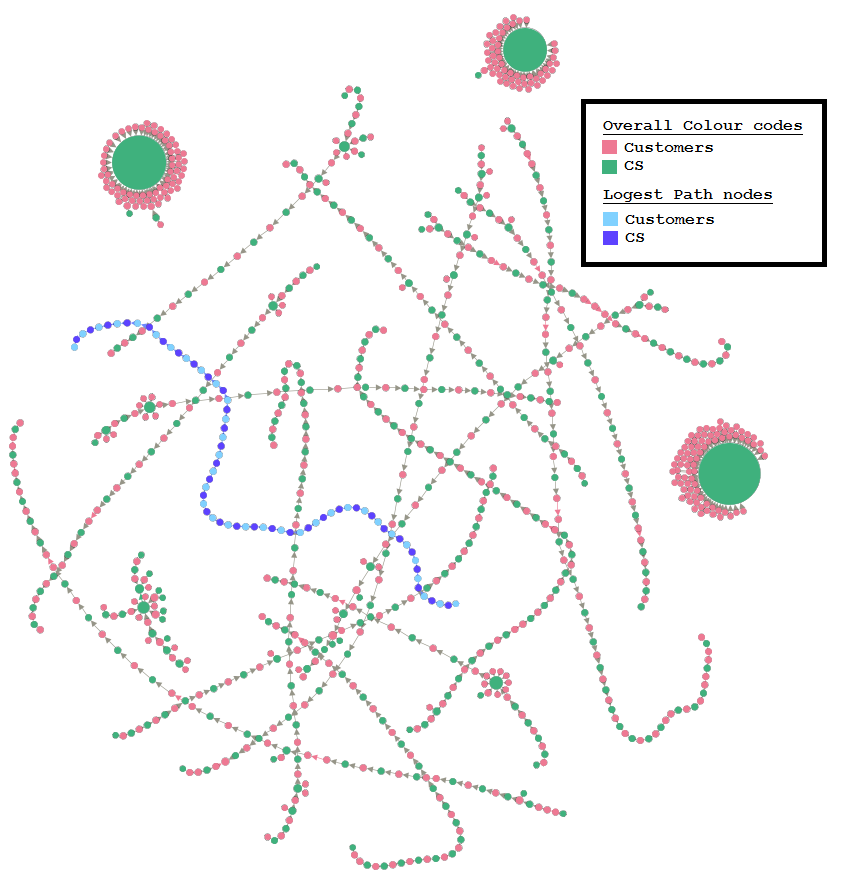
\includegraphics[width=0.6\textwidth]{images/20ccpostpostgraph.png}
\caption{Largest 20 connected components in post-post graph}
\label{fig:20ccpostpostgraph}
\end{figure*}

Generally, simple chains can be identified where the number of edges
equals length of the longest path in component. Simple chains account
for 80\% of the connected components in graph, of which 47\% were
found with the length of 1. This is in agreement with the results of
connected component sizes presented earlier. Finally,
Table~\ref{tbl:delaystatscl} presents statistics on chains of
individual CS accounts.

% \begin{figure}[htb]
% \centering
% 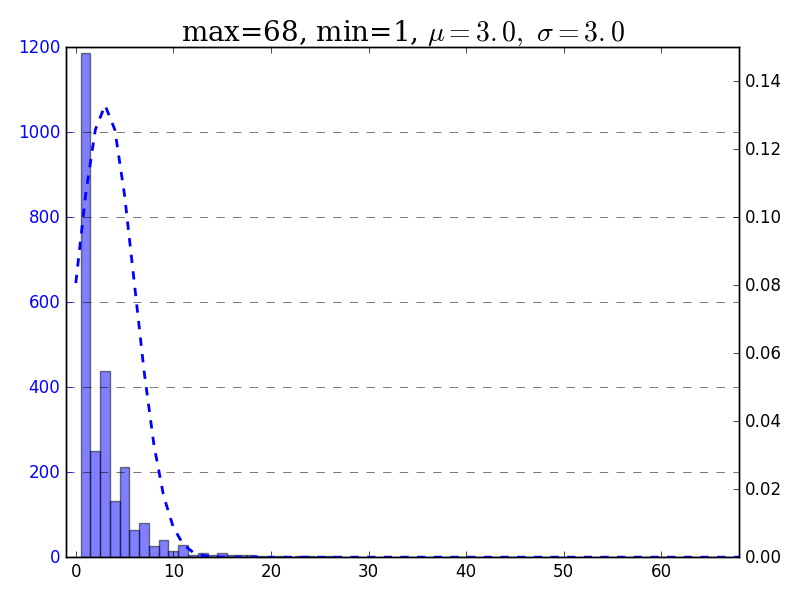
\includegraphics[width=\columnwidth]{images/simplechainlengths.png}
% \caption{Simple chain lengths}
% \label{fig:simplechainlengths}
% \end{figure}

\begin{table}[!h]
\centering
\begin{tabularx}{\columnwidth}{lrrrrr}
\toprule
\textbf{Name} & \textbf{count} & \textbf{max} & \textbf{min} & \textbf{mean} & \textbf{stdev}\\ 
\midrule
{\emph{btcare}} & 388 & 19 & 1 & 3.46 & 3.22\\
{\emph{ee}} & 324 & 9 & 1 & 1.98 & 1.43\\
{\emph{giffgagg}} & 147 & 12 & 1 & 2.39 & 1.98\\ 
{\emph{o2}} & 216 & 11 & 1 & 2.53 & 2.26\\
{\emph{skyhelpteam}} & 252 & 15 & 1 & 2.22 & 1.99\\
{\emph{virginmedia}} & 959 & 68 & 1 & 3.78 & 4.46\\
{\emph{vodaphoneukhelp}} & 248 & 39 & 1 & 2.58 & 3.29\\
\bottomrule
\end{tabularx}
\caption{Summary statistics on chain length for CS accounts}
\label{tbl:delaystatscl}
\end{table}

\subsection{Coexistence and Competition}

As presented earlier, connected components in the base graph represent
individual conversations. Therefore, those components were used to
uncover indirect engagement amongst CS accounts. As reply nodes in the
graph include the account name of the user, it is possible to identify
those components with more than one CS account. For each connected
component, the names in reply nodes are checked if they belong to a CS
account or not. Components with more than one distinct CS name are
then marked as coexistence component. The results show that there were
39 coexistence components in total; 38 include two CS accounts, and
one includes three accounts. The graph presented in
Figure~\ref{fig:commoncc} shows those components, with each CS account
given a colour code for identification as the legend clarifies.

\begin{figure*}[htb]
\centering
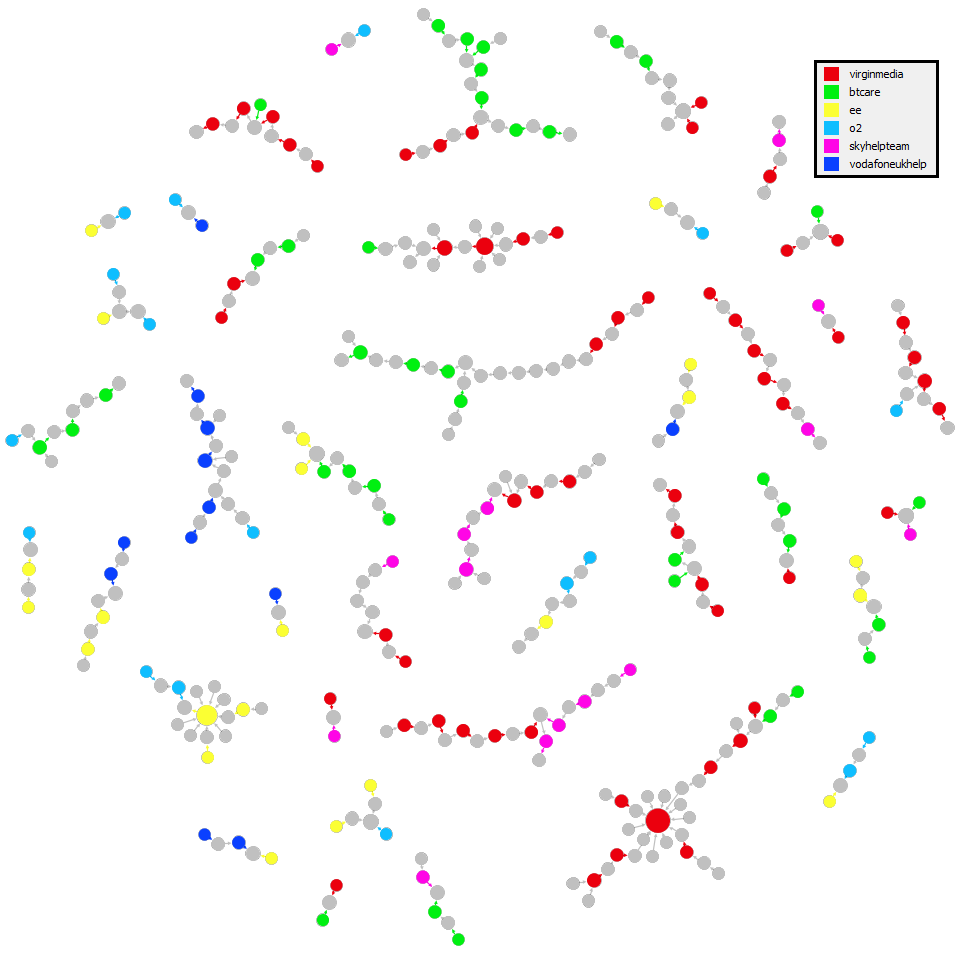
\includegraphics[width=0.6\textwidth]{images/commoncc.png}
\caption{Common connected components}
\label{fig:commoncc}
\end{figure*}

To explore these relationships further, a specific users graph was
constructed based on those components. Construction of this graph
follows similar steps as used in the customer-CS graph. However, as CS
accounts do not have direct engagement with each other, edges in this
graph are undirected and their weights indicate the number of times
they appeared together in the same conversation component.  The
resulted CS-CS graph is shown in Figure~\ref{fig:coexistencegraph},
where node size is proportional to its degree to indicate how many
other CS accounts the node has coexisted with, while darkness of node
reflects weighted degree to show the total frequency of coexistence
for the node.

The first observation on the graph is that {\emph{@giffgaff}} account
was not found in any common conversation. In contrast, {\emph{@o2}}
was the only account that have shared conversations with all other
selected CS accounts, while {\emph{@vodafoneukhelp}} was found with
the least common conversations. Nevertheless, weighted degree measure
shows that {\emph{@virginmedia}} was the highest in number of common
conversations -- 21 components -- although its degree tells that those
conversations were shared with only three other CS teams. The heaviest
edge existed between {\emph{@virginmedia}} and {\emph{@btcare}},
followed by the edge between {\emph{@virginmedia}} and
{\emph{@skyhelpteam}}. Also, edges of {\emph{@o2}} show that it mostly
appeared with {\emph{@ee}}, and for {\emph{@vodafoneukhelp}} it was
{\emph{@ee}}.

The observation of edges and their weights can provide insight into
uncovering more specific service areas within the specific industry or
sector. This was clear when the modularity of the graph was
examined~\cite{Blondel2008}; the result has unfolded into two
communities, as shown in Figure~\ref{fig:modularityclassgraph}. Also,
industry knowledge regarding the following CS teams: {\emph{@ee}},
{\emph{@o2}}, and {\emph{@vodafoneukhelp}} belong to a domain that is
mostly focused on mobile services, while {\emph{@skyhelpteam}},
{\emph{@virginmedia}}, and {\emph{@btcare}} are mostly known to be
focusing on landline and home internet services.

\begin{figure}[htb]
\centering
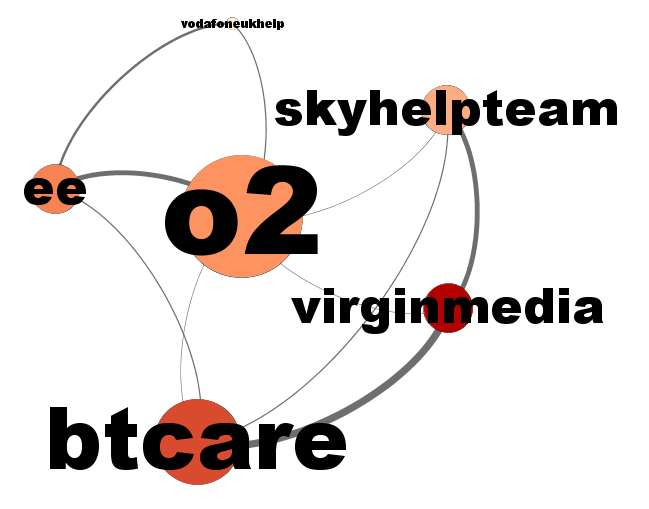
\includegraphics[width=\columnwidth]{images/coexistencegraph.png}
\caption{CS-CS coexistence graph}
\label{fig:coexistencegraph}
\end{figure}

\begin{figure}[htb]
\centering
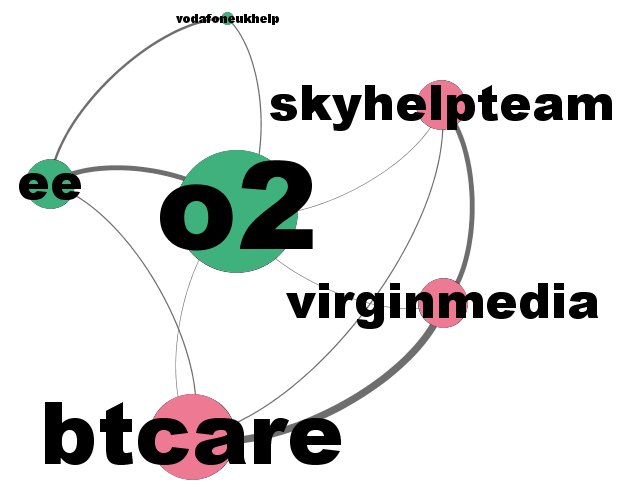
\includegraphics[width=\columnwidth]{images/modularityclassgraph.png}
\caption{Modularity class graph}
\label{fig:modularityclassgraph}
\end{figure}

Furthermore, using a similar approach that was used in
Section~\ref{results_delay}, the delay was measured in those
components to evaluate if presence of competitor has an influence on
the latency of the CS team response. Interestingly, an improvement in
delay of 26\%, 43\% and 72\% were observed for
{\emph{virginmedia}},{\emph{btcare}} and {\emph{skyhelpteam}},
respectively. These changes in delay, in addition to the frequency of
the companies common conversations presented earlier, confirm the
existence of online competition amongst them.

% \begin{figure}[htb]
% \centering
% 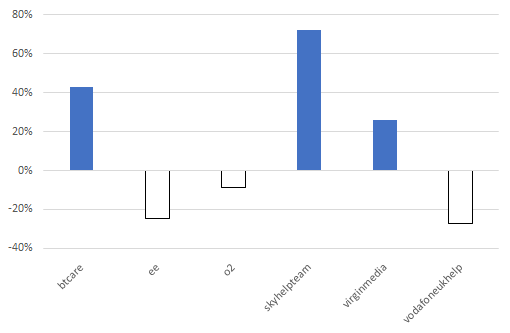
\includegraphics[width=\columnwidth]{images/diffdelaymeans.png}
% \caption{Modularity class graph}
% \label{fig:diffdelaymeans}
% \end{figure}

% To better understand the context of conversations in those common
% components, text analysis was carried out for each CS account. The
% attempt is a try to find what the customer have said that made the CS
% team participate in the conversation. Therefore, posts of CS accounts
% were eliminated, and the analysed texts include posts of customers
% only. Presentation of the result could be shown in table of statics,
% rather, wordcloud visualisation was used for each CS account. Initial
% results show that mentions were found very high in number. Therefore,
% another one was generated after removing mentions, results are
% presented in Figure ‎2.17.

% Interestingly, the first set of results (with mentions) provide
% explanation and insights on edge weights shown in
% Figure~\ref{fig:20ccpostpostgraph}. Taking one example, the edge
% {\emph{virginmedia}}--{\emph{btcare}} was found the heaviest. However,
% the first set of wordclouds for both show that {\emph{virginmedia}}
% was the mostly mentioned by customers. Same conclusion was found for
% the edge {\emph{skyhelpteam}}--{\emph{virginmedia}}.

% The other set, with mentions removed, may be used to identify some
% keywords for what could possibly be main issues, problem, or complains
% that might be of advantageous to other business rivals.


\section{Discussion}\label{discussion}

Initially, the performance of CS accounts and their popularity on
Twitter were measured by an analysis of activity and users. From this
perspective, {\emph{@virginmedia}} was found to have the highest
volume of posts, the least diverse in terms of type of posts (99.7\%
were replies) and with the highest number of customers served. The
average delays of accounts ranged between 1.14 and 3.34 hours, apart
from {\emph{@skyhelpteam}} which was found with an average delay of
45.04 hours. This may indicate a management issue for the team, such
as unclear social media strategy or staff resources.

Most CS teams have clearly specified working hours on their account
page, apart from {\emph{@giffgaff}} and {\emph{@o2}}. Interestingly,
these two accounts were found to have the lowest delay. Nevertheless,
high availability, i.e. longer activity hours, was not found to
significantly improve speed of reply to customers. For example, while
{\emph{@giffgaff}} was observed active for longer periods, {\emph{@o2}}
was generally found to be faster to reply.

Although the data shows that no CS team has been in a direct
engagement with a competitor, analysis of common/shared connected
components has uncovered some form of competition amongst CS
accounts. Particularly, in the case of {\emph{@virginmedia}} and
{\emph{@btcare}}, the competition was clear and intense. In all cases,
customers were found to be initiators of competing conversations by
making use of the Twitter {\emph{@-mention}} feature to bring
different rivals into conversations. In contrast to phone, letter or
email, complaints that are made on social media are open for the
public to read and follow, and can be potentially reputationally
damaging if not handled appropriately. Therefore, it was not
surprising to see improvement in the speed of response in a few
instances where competitors were included in the same
conversation. This shows that with the openness of social media
platforms, such as Twitter, customers may have more chance to obtain
better deals or speedy resolution of their
problems~\cite{einwiller+steilen:2015}. In turn, this approach of
publicly-posting complaints add pressure onto CS teams to improve
their social media engagement, especially when business rivals are
included by customers~\cite{gregoire-et-al:2015}.

Some of these issues are particularly pertinent for the mobile virtual
network operators (MVNOs) -- such as Virgin Mobile, giffgaff and Sky
Mobie -- who use the infrastructure of the main mobile network
operators (MNOs), as presented in Section~\ref{casestudy}. While this
may not directly affect CS operations, especially as many customers
are unlikely to be aware of whether their company owns any underlying
network infrastructure, it may have operational and/or performance
impacts on the virtual operators depending on their service-level
agreements with the infrastructure operators.

\section{Conclusions}\label{conclusions}

The paper has introduced an extensible framework for evaluating
customer service performance and competition between industry rivals
on Twitter. We have presented methods on how network graph properties
can be used to make increasingly sophisticated evaluations, with the
framework being tested on selected operators in the competitive UK
telecoms sector.

Section~\ref{method} highlighted two important techniques that need to
be applied prior to starting the analysis phase. First, the recursive
reply chain data collection is vital to obtain accurate results. The
importance of this stage stems from the fact that it fills the gaps
and improve the connectivity of graphs. Second, construction of the
initial graph from replies and the removal of floating isolated
nodes. In constructing this graph, key information needs to be
identified and attached as attributes to nodes. The information used
in this study include post {\emph{id}}, {\emph{timestamp},
{\emph{screen\_name}, {\emph{text}} and {\emph{CS}} value. However,
the framework could easily be extended to include other information,
such as retweets.

A wider aim of this project is to show the importance of connected
components in distinguishing users' conversations, as well as
analysing competitions and their key features. With the added value of
modularity classes, competition analysis has helped in uncovering more
specialist communities within the industry sector.

The presented framework could also be used by service providers to
reflectively evaluate their social media accounts and interactions, as
well as to generate insight into the activities of their key domain
competitors; in this way, the presented methods in this study could be
used to make real-time observations. Another application would be to
identify gaps, competitions, challenges and opportunities in services
that can be used in developing strategies for start-ups, for
example. The approach could also be applied to other domains or
contexts, such as non-profits, charities or the public sector. Also,
it can be used for groups of users, such as celebrities and their
direct and indirect engagements on Twitter. Moreover, with the
emerging practice of signing a reply with a team member's initials,
this practice can be exploited to further augment this framework's
capabilities; for example, this extension could help in estimating
team sizes, working shifts and to evaluate performance of individual
team members.

\section*{Acknowledgements}

This work has been supported by a doctoral research scholarship for
Nabeel Albishry from King Abdulaziz University, Kingdom of Saudi
Arabia.

\bibliographystyle{ACM-Reference-Format}
\bibliography{ssei2018} 

\end{document}
